%\documentclass[review]{elsarticle}
\documentclass[preprint,3p,11pt]{elsarticle}

\usepackage{hyperref}
\usepackage{xspace}
\usepackage{tabularx}
\usepackage{longtable}
\usepackage{array}
\usepackage{url}
\usepackage{fancyvrb}
\usepackage{listings}
\usepackage{courier}
\usepackage{graphicx}
\DefineShortVerb{\|}
%\usepackage{lineno}
%\modulolinenumbers[5]

\newcommand\userinput[1]{\textbf{#1}}
\lstset{basicstyle=\footnotesize\ttfamily,breaklines=true}
\lstset{framextopmargin=50pt,frame=bottomline}

\journal{Journal of Unpublished HAD Reports}

%%%%%%%%%%%%%%%%%%%%%%%
%% Elsevier bibliography styles
%%%%%%%%%%%%%%%%%%%%%%%
%% To change the style, put a % in front of the second line of the current style and
%% remove the % from the second line of the style you would like to use.
%%%%%%%%%%%%%%%%%%%%%%%

%% Numbered
%\bibliographystyle{model1-num-names}

%% Numbered without titles
%\bibliographystyle{model1a-num-names}

%% Harvard
%\bibliographystyle{model2-names.bst}\biboptions{authoryear}

%% Vancouver numbered
%\usepackage{numcompress}\bibliographystyle{model3-num-names}

%% Vancouver name/year
%\usepackage{numcompress}\bibliographystyle{model4-names}\biboptions{authoryear}

%% APA style
%\bibliographystyle{model5-names}\biboptions{authoryear}

%% AMA style
%\usepackage{numcompress}\bibliographystyle{model6-num-names}

%% `Elsevier LaTeX' style
\bibliographystyle{elsarticle-num}
%%%%%%%%%%%%%%%%%%%%%%%

\begin{document}

\begin{frontmatter}

\title{Implementing DANE Email Testers}
% \tnotetext[mytitlenote]{Fully documented templates are available in the elsarticle package 
% on \href{http://www.ctan.org/tex-archive/macros/latex/contrib/elsarticle}{CTAN}.}

%% Group authors per affiliation:
\author{Simson Garfinkel}

\begin{abstract}
DNS-Based Authentication of Named Entities (DANE) can be used to
improve the trustworthiness of email by providing a discovery
mechanism for certificates and public keys that are used to secure the  SMTP communications
between Mail Transfer Agents (MTAs) and to encrypt email. A testing
frameworks for each of these DANE applications was created. The SMTP
tester uses a conventional logic-driven approach for test
frameworks, while the OPENPGPKeys and SMIMEA testers employ a
database-driven testing framework that implements the tester as a
state machine. The two approaches are compared in terms of
development time, functionality, and extensibility.
\end{abstract}

\begin{keyword}
DNS-Based Authentication of Named Entities\sep DANE\sep OPENPGPKeys\sep SMIMEA
\end{keyword}

\end{frontmatter}

\tableofcontents

%\linenumbers

\section{Introduction}

Unprotected email that travels over the Internet is susceptable to monitoring and
alteration. There are two general approaches to securing email:
point-to-point encryption of the communications between email
servers, and end-to-end encryption of the individual email
messages. Because of the scale of the Internet, securing the email
infrastructure with a symmetric encryption is infeasible; only security systems based
on public key cryptography can be adequately scaled to match the task.

Applying Public key cryptography to securing email requires that participants have some mechanism
for discovering the public keys of their correspondents. Within a single organization,
an enterprise directory can be used to distribute public
keys, and traditional PKI mechanisms\cite{rfc5280} can be used to certify them. 

DNS-Based Authentication of Named Entities\cite{rfc7671} (DANE)
provides a general mechanism for the discovery of cryptographic keys
associated with objects that have names that can be expressed as
domain names, such as web servers. By relying on the DNSSEC\cite{rfc3833}
trust roots, DANE delegates control of the names within an
organization's DNS hierarchy to the administrative unit that is in
control of the organization's DNS. Thus, DANE transforms DNS into a
global directory for certifying identities.

Support for DANE has been added to OpenSSL (v. 1.1.0), GnuTLS
(v.3.5.4), and Postfix (v2.11). But properly implementing DANE requires not just conforming
software, but the generation and installation of cryptographic
materials (e.g. certificates and keys), the generation and installation of appropriate DNS
records, and the correct configuration of DNSSEC. An error or mismatch of any of these
objects might result in the inability to properly encrypt, sign,
validate, or deliver email. Thus, there is a significant need for an
easy-to-use testing infrastructure that can be used to develop, debug
and certify both software and operational deployments, and this testing infrastructure
must be easy-to-update as the underlying specifications evolve.

\subsection{DANE for SMTP}

Although many SMTP servers now implement the STARTTLS SMTP
command\cite{rfc3207}, Mail Transfer Agents (MTAs) typically
accept certificates signed by \emph{any} Certificate Authority (CA),
as well as certificates that are self-signed. This promiscuous
approach to trust is called ``opportunistic encryption,'' and it is
supported on the grounds that it is generally better to use encryption
if the opportunity is provided than to not use encryption.

Opportunistic encryption provided by the STARTTLS command provides security
against a passive monitoring attacker. However, the casual acceptance
of certificates signed by any CA leaves unencrypted Internet email
susceptible to interception by an active attacker that can perform a
man-in-the-middle attack. Such attacks can be readily performed by
manipulating DNS responses or routing protocols.

RFC7671\cite{rfc761} and RFC7672\cite{rfc7672} provide a mechanism for SMTP clients to discover
information that allows the certification of an SMTP server's public
key. Thus, while DANE cannot prevent
man-in-the-middle attacks, it does provide allow an MTA 
to determine that a man-in-the-middle attack is taking place. Once
detected, the server can refuse to send email. Sadly, there is no way
for an MTA to distinguish between a man-in-the-middle attack and a
misconfigured server.

\subsection{DANE for Email Encryption}

End-to-end encryption of email messages is complicated by the fact
that more than two decades of research and standards development
has produced two 
standards for the exchanging encrypted Internet email that are both
deployed and mutually incompatible:
S/MIME\cite{rfc5750} and OpenPGP\cite{rfc4880}. Before the advent of
DANE, there was no standardized mechanism for a sender to reliably obtain the
public key for an intended recipient. We call this the \emph{key
  discovery problem}. S/MIME mitigates this problem somewhat,
as digitally signed S/MIME messages typically have the sender's public
key embedded in the PKCS\#7 attachment\cite{rfc2315}. Thus, S/MIME
correspondents will frequently exchange clear-text but digitally
signed messages as prelude to exchanging encrypted email. OpenPGP
attempted to solve the key discovery problem with the PGP Key
Servers, and by organizations publishing their PGP Public Keys on
their websites. 

Work is in progress on a mechanism that use DANE for discovering S/MIME certificates
associated with email addresses (\emph{draft-ietf-dane-smime11}), and
an experimental RFC was recently approved that uses DANE for associating OpenPGPKey
public keys with email addresses\cite{rfc7929}. With these mechanisms,
the sender of an email can fetch the recipient's S/MIME certificate or
PGP public key and send that the recipient an encrypted message,
without the need to first exchange a message that is digitally signed.

\subsection{Our Contribution}

We created a tester for DANE-enabled HTTP and SMTP servers. The
tester, written in Python 2.7, includes an instrumented DANE
implementation that acquires the DANE DNS Resource Record(s) (RR(s)) for
either an HTTP or SMTP server and compares these RR(s) with the service
certificate associated with the HTTP or SMTP server. The tester can be run from
the command line or a web interface. Testing results are incorporated into
a data structure which can then be rendered as either text or HTML.

The server tester was implemented using commonly accepted
programming practices including object-oriented design,
modularization, and integrated tests. Nevertheless, the author found
it difficult to develop, audit, and extend the tester to new protocols. A 
complicating factor is that a successful DANE validation depends on both the server's certificate and the results of DNS
queries, but DNS servers frequently give different answers to the same
questions as a result of caching, load balancing, network congestion,
and configuration changes. Thus, it was frequently difficult to
determine to replicate the tester's verdict regarding the correctness
of an organization's DANE deployment.

Following the development of the first tester, we created a
tester for the draft SMIMEA and OpenPGPKey protocols. The second
tester was based on the core ideas of \emph{repeatability} and \emph{auditability},
which we define as ``the degree to which transactions can be traced
and audited through a system.'' A design requirement of the second tester  was to maintain a log of all DNS queries and responses
so that the tester's edicts could be reviewed and validated. Another
design goal was to enable a \emph{replay} capability, so that previous
queries and responses could be used for regression testing. In the
process of designing the new testing framework, we implemented the entire
testing framework as a state machine, with each phase
of the test corresponding to states and state transitions being
directed by the responses from the system undergoing test. This design
change resulted in superior decomposition of the testing system,
resulting in code that was easier to validate and audit.

\subsection{Availability}

The complete DANE tester is available from Github at
\url{https://github.com/usnistgov/dane_tester}. Both testers are
operational at \url{https://dane-test.had.dnsops.gov}


\section{Prior Work}
Automated protocol testing is a longstanding goal in network design
and development. Much of the literature explicitly uses finite state
machines to model the test process and applies formal methods to
discover new test cases.

In 1983, Sarikaya and Bochmann modeled network protocol as a
stimulius/response sequence, and developed algorithms for generating
test sequences to allow for automated testing of network
protocols\cite{Sarikaya:1983:SIP:1024840.1035264,Sarikaya:1983:SIP:1035237.1035264}.
Follow-up work by Sabnani and Dahbura explicitly modeled protocols as
a finite state machine\cite{Sabnani:1985:NTG:319056.319003,Sabnani:1985:NTG:318951.319003}.

Bochmann and Petrenko reviewed more than a dozen methods available for protocol testing
in 1994~\cite{Bochmann:1994:PTR:186258.187153}. They discussed options
for using specification languages for communications protocols,
approaches for testing using Finite State Machine specifications,
fault injection, and approaches for deriving tests from FSMs.

Model checking emerged in the late 1990s as lightweight approach for
using formal methods. An advantage of model checking was it allowed a
large state space to be explored fairly quickly. While not exhaustive,
model checking frequently found errors that were not found either by
manual testing or by more traditional formal methods.

In 2006 Maag et al.\ proposed using model checking for conformance testing and
verification of protocols~\cite{Maag:2006:TMA:1163653.1163663}. In 2009 Fan et al.\ developed a protocol tester based on Finite State Machine
(FSM) theory~\cite{Fan:2009:PPT:1582379.1582477}. Also in that year,
Bertolino et al.\ applied automated methods and model checking to
testing web services\cite{Bertolino:2009:ASB:1595696.1595719}. And Pike presented an approach for building protocol testers using the
Haskell programming language\cite{Pike:2009:RYO:1596638.1596646}. Two
years later, Wang et al.\ discussed automated approaches for bringing testers to rarely
entered parts of protocol~\cite{Wang:2011:ADP:2069131.2069166}.

More recently, Tulpule describes the Google+ team's approach to testing the
interaction between mobile clients and
servers~\cite{Tulpule:2013:STC:2542128.2542134}. The system creates
tests by recording the behavior of actual clients and then replying them
against a server. 

\section{HTTP and SMTP Server TLSA Tester}
We created a tool to test server certificates advertised using DANE
for availability, validity and protocol conformance. The server tester
tests both HTTP and SMTP servers, and can easily be adapted to servers
for other SSL-based protocols should they become available.

\subsection{Overview}

The tool compares the certificates provided by the
SSL server(s) associated with a webserver or email server are
consistent with the records provided by one or more DNSSEC TLSA
RRs. It does so by following these rough steps. 

\begin{enumerate}
\item The user specifies a service to test (either an HTTPS URL or an
  email address).
\item Using getdns, the tester obtains the DANE announcements for the
  service. 
\item The tester connects to the service and reports if the server's
  public key is validated by any of the   certificates or public keys
  advertised through DNS TLSA records. 
\end{enumerate}

To perform these tests, the tester contains its own DANE
implementation. The implementation covers several specific cases,
including:

\begin{itemize}
\item If the DNS name maps to multiple IP addresses, each IP address
  is tested. (Different IP addresses may have different certificates.)
\item If the DNS name specifies a CNAME, the CNAMEs are followed until
  the end of the change. A DANE record is looked for both the original
  DNS name and the name pointed to be the CNAME chain.
\item If the mail delivery host specifies a mail exchanger (MX)
  record, then both the primary name and the exchangers are tested.
\end{itemize}

\subsection{System Requirements}

\begin{description}
\item[OpenSSL v 1.0.2h]
The TLSA tester tests certificate validity using the \verb+openssl+
command line program, which is called using Python's \verb+subprocess.Popen()+
facility. Testing requires the flags |-purpose|, |-trusted_first|,
|-partial_chain| and |-CAfile|. These flags are only available on
OpenSSL version 1.0.2h and above.

Because US Government deployments are likely to have the
most recent FIPS-140 accredited OpenSSL version installed, which is
currently OpenSSL version 0.9.8zh, the installing scripts download and
install a private copy of OpenSSL version 1.0.2h in the
\verb+/usr/local/ssl+ directory.

\item[Python 2.7]
The TLSA tester also required that Python modules \verb+getdns+ and
\verb+M2Crypto+ be installed. The only version of Python that supports
both is Python 2.7, so these modules are added to the Python 2.7
installation, even if a version of Python 3 is installed.

\item[M2Crypto] The Python package M2Crypto is used for some
certificate manipulations.

\item[getdns] The TLSA tester uses getdns and Verisign's getdns Python
bindings. Numerous problems resulted from the decision to use getdns
and it was not used in the follow-on tester.

\item[py.test] The Python test framework \texttt{py.test} is used
for unit tests. Be sure to use version Python 2.7.
\end{description}

\subsection{File Layout}

The tester is contained entirely in the {\tt server/} directory of the
git repository. It is implemented as a Python module and a CGI
script. The tester consists of the following shown in Table~\ref{tlsa}.

\begin{table*}
\fbox{\begin{tabularx}{\textwidth}{>{\tt}lX}
file & purpose\\
\hline
Makefile & Targets for configuring Centos 7 base system and compiling helper programs. \\
README.md & Documentation \\
ca-bundle.crt & File containing multiple PEM-encoded SSL certificates of ``Well known'' Certificate Authorities. Used for Certificate Usage 0, which validates against system trust anchors. \\
centos7-setup.bash & Script to configure Centos 7 system to run the tester. \\
dane\_check.cgi & CGI script to run the tester from a webserver.\\
dane\_checker.py & Python module that implements DANE tester. Called by dane\_check.cgi and runnable directly from the command line. Can output both TEXT and HTML data.\\
dnstree.py & A program to test the getdns system.\\
get\_altnames & The compiled executable for the \emph{get\_altnames.c} program.\\
get\_altnames.c & M2Crypto provides no mechanism to read the alternative names on the X509 certificate, so this helper program gets the alt names of a certificate provided on the command line and prints the names to stdout.\\
test\_dane.py & A test program using the py.test framework to test functions within the {\tt dane\_checker} module.\\
\end{tabularx}}
\caption{Files in the \texttt{server/} directory}\label{tlsa}
\end{table*}

\subsection{System Preparation}

Preparing the system for the DANE server tester is complicated by the
tester's use of getdns. The version of getdns that is distributed with
Centos7 has a bug that prevents the verification of DNSSEC signatures
on CNAME RRs. Unfortunately, the version of getdns on the download
site does not compile with the version of Unbound that is in the
Centos7 ``yum'' package repositories. Therefore it is necessary to
download and install unbound and getdns. A further complication is
that the current version of getdns (getdns-1.0.0b2) requires the
\#include file |unbound-event.h|, which the unbound installer does not
install by default. 

Another complication is that the server tester requires a 
version of OpenSSL more recent than 1.0.2h. However, we could not get
getdns to compile with this version. Thus it is necessary to install
unbound and getdns, and then install OpenSSL 1.0.2h in a non-standard
directory (we chose the default installation directory,
|/usr/local/ssl|). 

The installation program |centos7-setup.bash|
addresses some of these issues, but we are not coding around all of
them in the hope that the unbound and getdns distributions will be
fixed. The script is idempotent, meaning that it can be re-run without
causing harm. This is especially useful if an action fails due to an
external cause, such as the inavailability of a repository.


\begin{enumerate}
\item Uncomment \texttt{AddHandler cgi-script .cgi} in the webserver's
  configuration file.
\item Add \texttt{ExecCGI} to the \texttt{Options} directive in the
  webserver configuration file.
\item Run the |centos7-setup.bash| script.
\item Set \verb|$DANESRC| to root of the cloned git repository.
\item Run the script |$DANESRC/server/centos7-setup.bash| %$ to install 
  the major Centos library modules that you need.
\item The script will stop. 
\item Download and install the current versions of unbound. Install
  the additional header directory |unbound-event.h|.
\item Download and install getdns.
\item Rerun the script |$DANESRC/server/centos7-setup.bash| %$
  to complete the installation.
\end{enumerate}

\emph{Note: On the github forum, the maintainers of getdns assert that
getdns should compile with the stock Centos7 unbound any version of
OpenSSL, and further state that the OpenSSL should be specified with
the \texttt{--with-ssl=} configuration option, rather than using the
\texttt{-I} and \texttt{-L} compiler flags to specify the location for the include
files and the library, respectively. This assertion has not been tested.}

\subsection{Installation and Operation}

The DANE server tester can be run from the command line using the
|dane_checker.py| script or from a web browser by placing the
|dane_check.cgi| script and the associated files in a
CGI-enabled directory of a modern web server. By design, the entire
GIT repository can be cloned in the directory of the web server.

\begin{enumerate}
\item Set \verb|$DANESRC| to root of the cloned git repository
\item \verb|cd $DANESRC|
\item Run |make| to compile |get_altname|.
\item Run |py.test| to run the self-test.
\item Run |python2.7 dane_checker.py https://good.dane.verisignlabs.com| to test Verisign's known-good
  DANE https server.
\item Run |python2.7 dane_checker.py https://bad-sig.dane.verisignlabs.com| to test one of Verisign's
  known-bad DANE https servers.
\item Run |python2.7 dane_checker.py --test| to test all of the test vectors.
\item Access \texttt{https://\emph{host}/\emph{directory}/dane\_check.cgi} to run
  the web-based tester
\end{enumerate}


\subsection{Theory of Operation}

To test a DANE server, the Python file |dane_checker.py| contains a
DANE implementation in Python. The test is coded as a series of
imperative statements that determine the name of the remote server,
perform DNS lookups to discover the IP address(es) on which the server
is running, fetch the server certificates, and then compare the server
certificates to the DNS announcements. 

Rather than printing out the results of the tests as they happen, the
testing infrastructure creates a data structure that contains a record
of each test that was performed and the results of the test. The
data structure can then be rendered as text or HTML as required by the
caller. 

The tests were developed by a
close reading of the DANE specifications. Each test is given a name
and a number. Each test description is then stored its own Python
object. The slots of the object are shown in Figure~\ref{slots}; the
test numbers ranges are shown in Table~\ref{ranges}.
\begin{table}
\centering\fbox{\begin{tabularx}{\textwidth}{llX}
slot & type & description \\
num & int & Test number, assigned by the author.\\
desc & str & A description of the test, in English.\\
section & str & The section of the DANE RFC from which the test derives.\\
failed\_desc & str & What to print if the test fails.\\
recommendation & boolean & If the test is for a recommended usage, but not a mandatory usage.\\
\end{tabularx}}
\caption{Slots in the DaneTest object}\label{slots}
\end{table}

\begin{center}
\begin{longtable}{|>{\small}l>{\small}l>{\small}p{3.25in}|}
\caption[Tests for DANE Servers]{Tests for DANE Servers}\label{tests-dane-servers} \\
\hline \multicolumn{1}{|c}{\textbf{\#}} & 
       \multicolumn{1}{c}{\textbf{Name}} & 
       \multicolumn{1}{c|}{\textbf{Description}} \\ 
\hline 
\endfirsthead
\multicolumn{3}{|c|}{{\bfseries \tablename\ \thetable{} -- continued from previous page}}
\\
\hline \multicolumn{1}{|c}{\textbf{\#}} & 
       \multicolumn{1}{c}{\textbf{Name}} & 
       \multicolumn{1}{c|}{\textbf{Description}} \\ 
\hline 
\endhead
\hline \multicolumn{3}{|r|}{{Continued on next page}} \\ \hline
\endfoot
\hline \hline
\endlastfoot
\multicolumn{3}{|c|}{}\\
\multicolumn{3}{|c|}{\textbf{\large 101--104: DNS tests}} \\
101 & TEST\_CNAME\_NOERROR     & If at any stage of CNAME expansion an error is detected, the lookup of the original requested records MUST be considered to have failed.\\
102 & TEST\_CNAME\_EXPANSION\_SECURE      & if at
   any stage of recursive expansion an ``insecure'' CNAME record is
   encountered, then it and all subsequent results (in particular, the
   final result) MUST be considered ``insecure'' regardless of whether any
   earlier CNAME records leading to the ``insecure'' record were ``secure.''\\
103 & TEST\_TLSA\_PRESENT    & Any connection to the MTA MUST employ TLS authentication (SMTP Server must offer STARTTLS)\\
104 & TEST\_TLSA\_DNSSEC     & Any connection to the MTA MUST employ TLS authentication (SMTP Server must offer STARTTLS)\\
\multicolumn{3}{|c|}{}\\
\multicolumn{3}{|c|}{\textbf{\large 201-205: Server verification}}\\
201 & TEST\_SMTP\_CONNECT    & Any connection to the MTA MUST employ TLS authentication (SMTP Server must offer STARTTLS)\\
202 & TEST\_SMTP\_STARTTLS   & Any connection to the MTA MUST employ TLS authentication (SMTP Server must offer STARTTLS)\\
203 & TEST\_SMTP\_TLS        & Internet-Draft RECOMMEND[s] the use of ``DANE-EE(3) SPKI(1) SHA2-256(1)'' with ``DANE-TA(2) Cert(0) SHA2-256(1)'' TLSA records as a second choice, depending on site needs.\\
204 & TEST\_SMTP\_QUIT       & Internet-Draft RECOMMEND[s] the use of ``DANE-EE(3) SPKI(1) SHA2-256(1)'' with ``DANE-TA(2) Cert(0) SHA2-256(1)'' TLSA records as a second choice, depending on site needs.\\
205 & TEST\_EECERT\_HAVE     & Internet-Draft RECOMMEND[s] the use of ``DANE-EE(3) SPKI(1) SHA2-256(1)'' with ``DANE-TA(2) Cert(0) SHA2-256(1)'' TLSA records as a second choice, depending on site needs.\\
\multicolumn{3}{|c|}{}\\
\multicolumn{3}{|c|}{\textbf{\large 301-308: \textbf{Certificate verification}}}\\
301 & TEST\_SMTP\_CU         & Internet-Draft RECOMMEND[s] the use of ``DANE-EE(3) SPKI(1) SHA2-256(1)'' with ``DANE-TA(2) Cert(0) SHA2-256(1)'' TLSA records as a second choice, depending on site needs.\\
302 & TEST\_TLSA\_CU02\_TP\_FOUND & Internet-Draft RECOMMEND[s] the use of ``DANE-EE(3) SPKI(1) SHA2-256(1)'' with ``DANE-TA(2) Cert(0) SHA2-256(1)'' TLSA records as a second choice, depending on site needs.\\
303 & TEST\_TLSA\_PARMS      & Internet-Draft RECOMMEND[s] the use of ``DANE-EE(3) SPKI(1) SHA2-256(1)'' with ``DANE-TA(2) Cert(0) SHA2-256(1)'' TLSA records as a second choice, depending on site needs.\\
304 & TEST\_TLSA\_RR\_LEAF    & Internet-Draft RECOMMEND[s] the use of ``DANE-EE(3) SPKI(1) SHA2-256(1)'' with ``DANE-TA(2) Cert(0) SHA2-256(1)'' TLSA records as a second choice, depending on site needs.\\
305 & TEST\_DANE\_SMTP\_RECOMMEND  & Internet-Draft RECOMMEND[s] the use of ``DANE-EE(3) SPKI(1) SHA2-256(1)'' with ``DANE-TA(2) Cert(0) SHA2-256(1)'' TLSA records as a second choice, depending on site needs.\\
306 & TEST\_EECERT\_VERIFY   & When name checks are applicable (certificate usage DANE-TA(2)), if
   the server certificate contains a Subject Alternative Name extension
   ([RFC5280]), with at least one DNS-ID ([RFC6125]) then only the DNS-
   IDs are matched against the client's reference identifiers.... The
   server certificate is considered matched when one of its presented
   identifiers ([RFC5280]) matches any of the client's reference
   identifiers.\\
308 & TEST\_DANE2\_CHAIN     & SMTP servers that rely on certificate usage DANE-TA(2) TLSA records for TLS authentication MUST include the TA certificate as part of the certificate chain presented in the TLS handshake server certificate message even when it is a self-signed root certificate.\\
\multicolumn{3}{|c|}{}\\
\multicolumn{3}{|c|}{\textbf{\large 401-407: Ensemble results}}\\
401 & TEST\_TLSA\_CU\_VALIDATES &  ``Domains that want secure inbound mail delivery need to ensure that all their SMTP servers and MX records are configured accordingly.'' Specifically, MX records that do not have DANE protection should not preempt MX servers that have DANE protection.\\
402 & TEST\_TLSA\_ATLEAST1   &  ``Domains that want secure inbound mail delivery need to ensure that all their SMTP servers and MX records are configured accordingly.'' Specifically, MX records that do not have DANE protection should not preempt MX servers that have DANE protection.\\
403 & TEST\_TLSA\_ALL\_IP     &  ``Domains that want secure inbound mail delivery need to ensure that all their SMTP servers and MX records are configured accordingly.'' Specifically, MX records that do not have DANE protection should not preempt MX servers that have DANE protection.\\
404 & TEST\_TLSA\_HTTP\_NO\_FAIL &  ``Domains that want secure inbound mail delivery need to ensure that all their SMTP servers and MX records are configured accordingly.'' Specifically, MX records that do not have DANE protection should not preempt MX servers that have DANE protection.\\
405 & TEST\_DNSSEC\_ALL      &  ``Domains that want secure inbound mail delivery need to ensure that all their SMTP servers and MX records are configured accordingly.'' Specifically, MX records that do not have DANE protection should not preempt MX servers that have DANE protection.\\
406 & TEST\_ALL\_SMTP\_PASS   &  ``Domains that want secure inbound mail delivery need to ensure that all their SMTP servers and MX records are configured accordingly.'' Specifically, MX records that do not have DANE protection should not preempt MX servers that have DANE protection.\\
407 & TEST\_MX\_PREEMPTION   &  ``Domains that want secure inbound mail delivery need to ensure that all their SMTP servers and MX records are configured accordingly.'' Specifically, MX records that do not have DANE protection should not preempt MX servers that have DANE protection.\\
\end{longtable}
\end{center}


































When |dane_checker.py| loads the \emph{DaneTest} objects are created
and stored in an associative array.

As the test program executes, traditional imperative logic implements
the DANE client and tests the server for correct responses. Whereas a
traditional tester might simply print the results, this tester instead
creates a list of \emph{DaneTestResult} objects. This list gets longer
as the test progresses towards completion. Most of the tester's
functions return a list of \emph{DaneTestResult} objects, which are
then concatenated to form the final result.

The \emph{DaneTestResult} object is a data structure that contains
structured information about whether each test passes or fails. For
example, the code shown in Figure~\ref{snipped-pem} calls |pem_verify|
to determine if an EE certificate verifies or not, and then stores the
results in a |DaneTestResult| object. A list of several such objects
is returned by the function. The slots of the object are shown in table~\ref{testResults}.



\begin{table}
\centering\fbox{\begin{tabularx}{\textwidth}{llX}
slot & type & description \\
\hline
passed & boolean & True if the test passed \\
dnssec & boolean & True if the test was a DNS lookup and the result was secured with DNSSEC \\
dnsrelied & boolean & True if the DNS lookup was relied upon. (Some DNS lookups may not be relied upon. For example, a DNS name may map to two IP addresses, but only one may have a functioning server.)\\
hostname & str & The relevant hostname.\\
ipaddr & str & The relevant IP address \\
test & DaneTestResult & A reference to the (immutable) \emph{DaneTestResult} object that corresponds to the test.\\
what & str & The context of what was being tested when the test took place.\\
rdata & str & The DNS response data (which the getdns API calls rdata) that was used in the test, if the test involves a DNS query.\\
key & str & Additional information returned in a DNS query, such as an
MX preference or a DANE cryptographic key. \\
\end{tabularx}}
\caption{DaneTestResults Object}\label{testResults}
\end{table}

How this works is illustrated in this snippet of code from the
function \emph{get\_dns\_ip} which is executed after an DNS query for
an MX RR, shown in Figure~\ref{snippet}. 

\begin{figure}
\begin{lstlisting}
    r = pem_verify(anchor_cert,cert_chain,certs[0])
    ret += [ DaneTestResult(passed=r,
                            test=TEST_EECERT_VERIFY,
                            hostname=hostname0,ipaddr=ipaddr,
                            what="Checking EE Certificate '{}'
                            against {}".format(cn,against)) ]

\end{lstlisting}
\caption{An excerpt of the logic used by the DANE Server Tester to
  verify a PEM certificate against and record the results.}\label{pem-snippet}
\end{figure}


\begin{figure}
\begin{lstlisting}
if a['type'] == getdns.RRTYPE_MX == request_type:
    what = 'DNS MX lookup {} = {} {}'.format(hostname,rdata['preference'],rdata['exchange'])
    ret.append( DaneTestResult(passed=SUCCESS,
                               what=what,
                               dnssec=reply.get('dnssec_status'),
                               rdata=rdata,
                               data=rdata['exchange'],
                               key=rdata['preference']))
\end{lstlisting}
\caption{An excerpt of the logic used by the DANE Server Tester to
  record the results of a DNS lookup of an MX record }\label{snippet}
\end{figure}

In this example, \emph{ret} is an array of \emph{DaneTestResult}
objects that will be returned. If an MX record is returned in the DNS
lookup, it's fields a broken out and added to \emph{ret[]}. DNS can
return multiple RRs in a query, and all of them are stored in
\emph{ret[]}.  They can then be both used in later parts of the test
and rendered for final output.

\subsection{Demo}
The tester is installed on the server dane-test.had.dnsops.gov. The
web page \url{http://dane-test.had.dnsops.gov/dane-tester/server/} is installed in the
directory |/var/www/html/dane-tester/server|.

\section{SMIMEA and OpenPGPKey Database-Driven Tester}
In addition to storing trust information for SSL servers, DANE now
supports the storing of S/MIME certificates and OpenPGP and public keys. This use
of DANE makes it possible for a DANE-aware Mail User Agent (MUA) to
fetch certificate or public key associated with an email address,
making it possible to send encrypted email and to verify digitally
signed mail without the need to use a Public Key Infrastructure (PKI)
or to obtain certificates through a manual process.

We created a tester for SMIMEA and OpenPGPKey protocols. The goal of
these tests was to implement an end-to-end test of mail systems that
use SMIMEA and OpenPGPKey. Thus, in addition to obtaining and verify
keys, the testers needed to be able to send encrypted mail and to
receive and verify digitally signed mail. In total, the 
SMIMEA and OpenPGPKey testers require the following functionality:

\begin{itemize}
\item Finding and fetching the S/MIME certificate or OpenPGP public
  key associated with an email address using the SMIMEA or OpenPGPKey
  protocol.
\item Encrypting a message using S/MIME or PGP.
\item Sending email messages that are not encrypted or encrypted.
\item Automatically processing incoming email messages.
\item Determining if an email message is signed and verifying the
  corresponding signature. 
\end{itemize}

\noindent Based on our experience in developing and using the server tester, we
had additional requirements on the test infrastructure:

\begin{itemize}
\item Track each test, including when the test started, completed, and
  all activity (e.g. DNS queries) associated with each test.
\item Capture the full contents of all DNS queries, so that they could
  be evaluated at a later point in time.
\item Maintain statistics of tester activity, and easily generate the
  statistics on demand.
\end{itemize}

\noindent Given these requirements, we decided to create a new framework for the
tester:

\begin{itemize}
\item Instead of controlling the test progression with a series of
  declarative statements, the new tester would implement each
  step in the test as state in a finite state machine. 
\item Each DNS query would be recorded and logged in the database,
  which would record the time the query was made, the query sent to
  the server, and the server's response. 
\item The single testing infrastructure should support multiple \emph{test
  types}. The database should record all of the steps associated with
  every invocation of a test type by a user, which we call a
  \emph{test instance}.
\item Each test type is given a unique name and identifier. The test type
  consists of a sequence of steps.
\item Each test instance is given a unique identifier. 
\item A \emph{workqueue} keeps track of the state of each running test instance.
\item Because this tester can send email, the tester requires that
  users register to prevent abuse. Registrations are stored in the
  database. Users are identified by email addresses and authenticated
  with a randomly generated password (called a \emph{hash} for
  historical reasons, even though it is not a hash). 
\end{itemize}

\subsection{Overview}
The database-driven tester is implemented with an object-oriented
Python framework, a set of command-line programs and CGI scripts, and
a MySQL database. Currently SQL statements are embedded directly in
the code, although the system could be modified to use an object
relation mapper (ORM) framework. 

\subsection{System Requirements}

\begin{description}
\item[OpenSSL] is used to implement S/MIME encryption and
signatures. The system was tested with version 1.0.2h, although any
version of OpenSSL should work that is more recent than 0.9.8n and
1.0.0 [29 Mar 2010], since there have been no changes made to the
S/MIME implementation since then according to the OpenSSL changelog. 

\item[python3] is used as the implementation language. This
implementation was tested with Python3.4 and Python3.5. 

\item[MySQL] is used as the database. We used MySQL version 5.1,
although any modern version should work. 

\item[pymysql] is used to prepare and send the embedded SQL
statements to the MySQL server.

\item[gpg] is used to implement the GPG encryption
algorithm. We tested with version 1.4.16.

\item[Python modules] The tester uses the Python modules PyMySQL,
dnspython, mako, and tabulate.
\end{description}

\subsection{Test Types and Database Layout}
The database-driven test system can support multiple different
\emph{test types}. Each test type is defined by a sequence of actions
that advance a test instance from test initiation to test
completion. The test types as of September 1, 2016 are shown in
table~\ref{testtypes}. 

Each test is fundamentally a finite state machine and consists of a
set of states and state transitions. Each state transition is
implemented as a named python function. Each test in progress is
stored within the MySQL database. The database also contains a record
of each state that the test has occupied, the current state, and the
arguments to supply to the next state transition function. The MySQL
database tables are presented in Table~\ref{db}. 

The database records all provenance associated with each test
instance. For example, instead of a single database row that records
the next state, multiple rows in the \emph{workqueue} table record,
for each test instance, each state through which the test instance has
passed, with a row indicating whether the state is pending or has been
completed. 

\begin{table}
\begin{center}
\begin{tabularx}{\linewidth}{lX}
\hline
name & description \\
\hline
bouncer   & This test receives an email message and sends a response. \\
dig       & This test performs a DNS lookup.\\
register  & This test allows a potential user to register an email address. \\
sendplain & This test sends a plain email message.\\
\hline
\end{tabularx}
\end{center}
\caption{Test types implemented by the database-driven test system.\ref{test-types}}
\end{table}


\begin{table}
\begin{tabular}{|>{\tt}llp{4in}|}
\hline
\textrm{table} & database keys & purpose \\
\hline
dns & dnsid, testid & Stores each DNS query and result. \\
keyencodings & keyencodingid & Stores encoding for S/MIME and OpenPGP keys. (Not currently implemented.) \\
messages & messageid, testid & Stores each email message sent or received, including full SMTP log (if available) \\
tests & testid, testtype & Provides a unique \texttt{testid} for each test that is initiated.\\
testtypes & testtype & Provides a unique name for each test type that is implemented by the system.\\
users & userid, email & Maps unique email addresses to unique |userid|s. For each email address tracks a username and the authentication ``hash.''\\
workqueue & workqueueid, testid & Tracks all actions scheduled and completed. Each work item is associated with a specific |testid| and has a set of arguments (|args|), stored as a JSON document.\\
\hline
\end{tabular}
\caption{MySQL Database tables used by the email tester.}\label{db}
\end{table}

\subsection{File and Class Layout}
The database-driven tester is implemented with an object oriented
framework, with the following classes and modules:

\begin{description}
\item[Tester] The primary class manages the database entries
created for each test instance. The |Tester()| constructor can be
called with a |testid=|, which creates a database connection for an
existing test instance, or without, in which case a new test instance
is created. A second parameter allows the created connection to be
read/write or read-only.

The |Tester| object reads the configuration file and creates a
connection to the MySQL database. If the |testid| was not provided, a
new test instance is created.O Once created, the |Tester| object is
passed to other functions and instances so that all of the
transactions associated with a specific test instance are connected
together.

\item[Dbdns] This module controls the database DNS
implementation. It contains functions that perform DNS queries,
records the results in the database, and returns the query. The
returned object  is compatible with the Python~3.2 |dnspython| API.

\item[smimea] This module implements the SMIMEA protocol. It contains
  functions to make an email message, to determine the DNS address
  corresponding to an email address, to get the certificate for an
  email address, and to use OpenSSL to digitally sign and/or encrypt
  an email message.

\item[openpgpkey] This module implements the OpenPGPKEY protocol. It contains
  functions to make an email message, to determine the DNS address
  corresponding to an email address, to get the certificate for an
  email address, and to use GPG to digitally sign and/or encrypt
  an email message.

\end{description}

\begin{table*}
\begin{tabularx}{\textwidth}{|>{\tt}lX|}
\hline
\textrm{file} & purpose\\
\hline
\multicolumn{2}{l}{\textbf{HTML files:}}\\
bootstrap/         & installation of Bootstrap HTML, CSS and JS framework.\\
index.html         & Home page for the tester.\\
jumbotron.css      & Bootstrap theme customization.\\
README.md          & The README program.\\
sendmail.html      & The HTML template used by the \texttt{email.cgi} script.\\
\\
\multicolumn{2}{l}{\textbf{Python Modules and Scripts:}}\\
cron\_runner.py    & Python script run by cron(8) to run the next step in the work queue.  \\
dbdns.py           & The database DNS implementation.\\
dbmaint.py         & The database maintenance program.\\
email\_receiver.py & A script that receives email messages and stores them in the database.\\
Makefile           & Stored commands for testing the test infrastructure.\\
msg-bounce.txt     & A test bounce message used for testing.\\
openpgpkey.py      & An OpenPGPKey implementation, uses \texttt{gnupg} command for cryptography..\\
periodic.py        & The workqueue runner.\\
schema.sql         & The database schema.\\
smimea.py          & An SMIMEA implementation, uses \texttt{openssl} command line for cryptography.\\ 
smtp.py            & An SMTP implementation that records all TCP interactions in the database.\\
tester.py          & The Tester class, which stores test results in the database, as well as configuration information.\\
\\
\multicolumn{2}{l}{\textbf{CGI Scripts:}}\\
email.cgi         & Allows the user to queue an email message.\\
history.cgi       & Allows users to see their interaction history with the tester.\\
lookup\_email.cgi & Allows users to look up a specific email message\\
lookup\_test.cgi  & Allows users to look up a specific test results.\\
sendmail.cgi      & Allows users to send an email message. \\
webcontrol.cgi    & \\
\hline
\end{tabularx}
\caption{Files in the \texttt{server/} directory}\label{server-files}
\end{table*}

\subsection{System Preparation and Installation}
The system preparation for the DANE server tester should also
installed the database-driven tester. Specifically, the script |server/centos7-setup.bash| will also install the necessary
Centos modules required to support the database-driven tester, and
Apache configuration that serves the |$DANESRC/server/| directory on
the web will also serve the |$DANESRC/email| directory. For our
production system, we simply cloned the |dane-test| git repository
into a directory that is served by the Apache web server. The file
|index.html| in the root directory gives web visitors the option of
running the DANE SSL client server or the email server. 

\subsubsection{Web files}

The tester uses Bootstrap as its HTML/JavaScript/CSS framework. To
install bootstrap, run |make install| from the root or the email directory. Make
sure that the Bootstrap is properly configured by displaying the
|email/index.html| page (see~\ref{email-home}).

\begin{figure}
\begin{center}
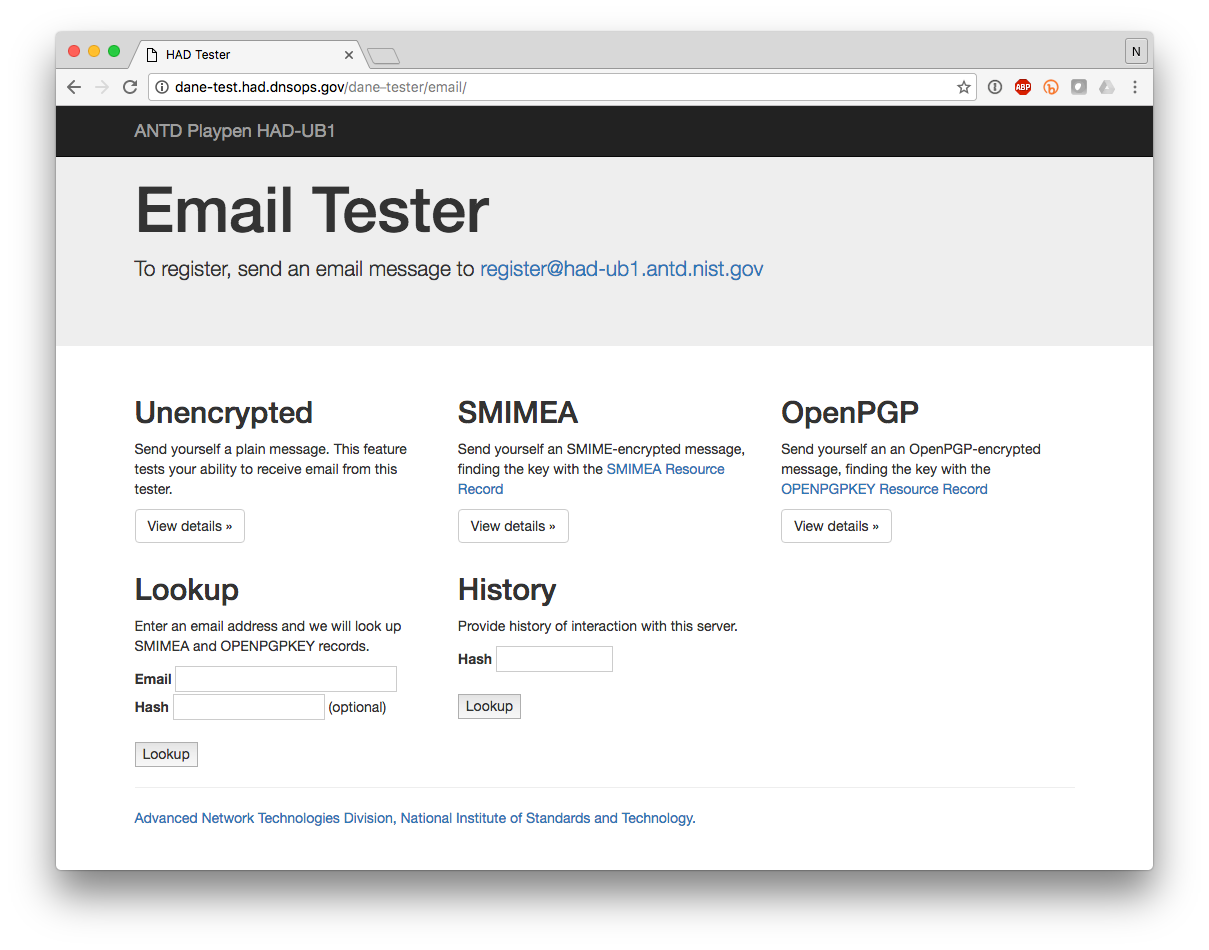
\includegraphics[width=6in]{email-home}
\end{center}
\caption{}\label{email-home}
\end{figure}

\subsubsection{Database Setup}

The database can be hosted on the same host as the server or on
another host. If the database is hosted on another Centos instance,
it will be necessary to open up the firewall on the database server
with the commands:

\begin{Verbatim}[commandchars=\\\{\}]
$ \userinput{sudo firewall-cmd --add-service=mysql}
$ \userinput{sudo firewall-cmd --permanent --add-service=mysql}
\end{Verbatim}

The testing framework requires a single database instance for its
tables. We recommend having two users that have access to the
instance: a database writer and a database reader. The current system
only supports the database writer user; the reader user will be used
at a later point for statistics.

On the database server, create the database user and the database that
will be used:

\begin{Verbatim}[commandchars=\\\{\}]
MariaDB [emaildb]> \userinput{create database emaildb;}
MariaDB [emaildb]> \userinput{create user 'dbwriter@129.6.100.204' identified by 'dbpassword';}
MariaDB [emaildb]> \userinput{grant all privileges on emaildb.* to 'dbwriter'@'dane-test.had.dnsops.gov';}
MariaDB [emaildb]> \userinput{grant all privileges on emaildb.* to 'dbwriter'@'%';}
MariaDB [emaildb]> \userinput{flush privileges;}
\end{Verbatim}

Be sure to test that you can connect to the database from the other host:

\begin{Verbatim}[commandchars=\\\{\}]
[db1]$ \userinput{mysql -udbwriter -pdbpassword -hdb1.antd.nist.gov emaildb }
MariaDB [emaildb]> \userinput{select version();}
+----------------+
| version()      |
+----------------+
| 5.5.50-MariaDB |
+----------------+
1 row in set (0.00 sec)
MariaDB [emaildb]> \userinput{quit;}
[db1]$ 
\end{Verbatim}

Once the database is created, it is necessary to load the schema into
the database. You can do this with the MySQL command:

\begin{Verbatim}[commandchars=\\\{\}]
[db1]$ \userinput{mysql -udbwriter -pdbpassword -hdb1.antd.nist.gov emaildb < email/schema.sql}
[db1]$
\end{Verbatim}

Once the database is created and connectivity is verified, the
connection information needs to be stored in the 
|email.cfg| configuration file. The information is stored in this file
so that the username and password do not need to reside in the source
code. \emph{This file should not be stored in the webserver
  hierarchy because it contains the database username, password, and
  host!} Instead, it should be stored in the home directory of the
user that runs the |cron_runner.py| script.

Here is a simple configuration file:

\begin{lstlisting}
[mysql]
username=dbwriter
password=dbpassword
dbname=emaildb
host=localhost
\end{lstlisting}

After the database is created and connectivity is created, a user
needs to be established that will run the scripts. As installed on
|dane-test|, the |slg| user runs the tester.   Install the configure
script in the user's home directory.

Next the tests need to be inserted into the database. This process
will also perform a test of the configuration file and the ability to
connect to the back-end database. Use the |dbmaint.py| command to
insert the tests and to test the installation with a database lookup:

\begin{Verbatim}[commandchars=\\\{\}]
$ \userinput{python3 dbmaint.py --create dig}
$ \userinput{python3 dbmaint.py --create register}
$ \userinput{python3 dbmaint.py --create sendplain}
$ \userinput{python3 dbmaint.py --list tests}
Tests:
  testtype  name
----------  ---------
        16  bouncer
        17  dig
        18  register
        19  sendplain
$
\end{Verbatim}
%$

\subsubsection{Configure for Sending and Receiving Email}

Additional configuration is required so that the tester can send and receive email

\paragraph{SMTP Server}

The SMTP server must be enabled and the server process must be
configured to listen to the appropriate interface. The default CentOS
configuration installs a \emph{postfix} process that only listened to
the |localhost| port. It is necessary to Edit the file
  \emph{/etc/postfix/main.cf} and modify the line |inet_interfaces| so
  that the server also listens on the \texttt{\$myhostname} interface:

\begin{Verbatim}[commandchars=\\\{\}]
inet_interfaces = $myhostname, localhost
\end{Verbatim}
%$

Be sure to restart the mail server after changes to this file

\paragraph{Firewalls.} The host-based firewall must be opened to allow the receipt of email:

\begin{Verbatim}[commandchars=\\\{\}]
$ \userinput{sudo firewall-cmd --add-service=smtp}
$ \userinput{sudo firewall-cmd --permanent --add-service=smtp}
\end{Verbatim}

It is also important be sure that the server's IP address and SMTP
port can be reached from the general internet. There may potentially
be many firewalls blocking access to port 25, including firewalls
operated by upstream providers, organizations, and VM
infrastructures. In our case, we had to clear firewalls operated by
our organization and our division.

\paragraph{Aliases}

Each address on which the tester receives email requires an entry in
the file |/etc/aliases| that directs the mail to the script. (Having a
script run when mail is received eliminates the need to poll for
delivered email.)  Currently we are using these two addresses:

\begin{Verbatim}[commandchars=\\\{\}]
### dane EMAIL tester:
bouncer:  ``|/var/www/html/dane-tester/email/email_receiver.py bouncer''
register: ``|/var/www/html/dane-tester/email/email_receiver.py register''
\end{Verbatim}

To test that email is being received, send a test registration message
to register@dane-test.had.dnsops.gov:

\begin{Verbatim}[commandchars=\\\{\}]
$ \userinput{mail register@dane-test.had.dnsops.gov}
Subject: Register Test
Register Me!
.
Cc:
$
\end{Verbatim}

Once the email is sent, its reception can be verified with the
|dbmaint.py| utility:

\begin{Verbatim}[commandchars=\\\{\}]
$ python3 dbmaint.py --list messages
Tests:
  messageid  fromaddr                                                  toaddr                                    
-----------  --------------------------------------------------------  --------------------------------------
        165  slg@dane-test.had.dnsops.gov (Basic)                      register@dane-test.had.dnsops.gov         
$
\end{Verbatim}

The workqueue can be viewed with the |--list workqueue| argument:

\begin{Verbatim}[commandchars=\\\{\}]
$ \userinput{python3 dbmaint.py --list workqueue}
Tests:
  workqueueid  modified             task                   testid  args                                   created                completed
-------------  -------------------  -------------------  --------  -------------------------------------  -------------------  -----------
          233  2016-09-07 09:58:20  register_from_email       342  {``cmd'': ``register'', ``messageid'': 165}  2016-09-07 09:58:20
$
\end{Verbatim}


In order to have the registration script run, it is necessary to have
system's |cron_runner.py| script run on a regular basis. We set the
script to run by the |cron| process every minute, by adding the
following lines to the user's cron script with the (e.g. ``crontab
-e'') command:

\begin{Verbatim}
#
# m h  dom mon dow   command
* * * * * /var/www/html/dane-tester/email/cron_runner.py
\end{Verbatim}

Note: be sure to add the |cron| command \emph{last!}

After the |cron_runner.py| script is running, the workqueue will
advance to indicate that the jobs have been run:

\begin{Verbatim}[commandchars=\\\{\}]
 $ python3 dbmaint.py --list workqueue
Tests:
  workqueueid  modified             task                   testid  args                                                                 created              completed
-------------  -------------------  -------------------  --------  ---------------------------------------------------------            -------------------  -------------------
          233  2016-09-07 16:21:01  register_from_email       342  {``cmd'': ``register'', ``messageid'': 165}                          2016-09-07 09:58:20  2016-09-07 16:21:01
          235  2016-09-07 16:21:01  crypto_message            342  {``state'': ``WORKING'', ``cmd'': ``register'', ``messageid'': 167}  2016-09-07 16:21:01  2016-09-07 16:21:01
          237  2016-09-07 16:21:01  send_message              342  {``state'': ``WORKING'', ``cmd'': ``register'', ``messageid'': 167}  2016-09-07 16:21:01
You have new mail in /var/spool/mail/slg
[dane-test ~/dane-tester/email 16:21:19](master) $
\end{Verbatim}

\subsection{Theory of Operation}

\subsection{Future Work}
\begin{itemize}
\item All configuration information should be moved out of tester.py
  and into email.cfg.
\end{itemize}

\section*{References}

\bibliography{rfc,fy16_report}

\end{document}

% LocalWords:  cryptographic modularization auditability exchanger MX changelog
% LocalWords:  inavailability unencrypted repeatability infeasible
% LocalWords:  misconfigured
